\chapter{Geometry}

\begin{definition}[Segments, Angles, and Directed Angles]
For points $A, B$, write $\overline{AB}$ for the segment and $AB$ for its length. The angle $\angle ABC$ has vertex $B$. For lines $\ell, m$ in the oriented Euclidean plane, $\angle(\ell, m)$ denotes their directed angle modulo $\pi$. In angle-chasing arguments, directed angles eliminate the need to distinguish many configurations involving interior and exterior angles.
\end{definition}

\begin{theorem}[Triangle Inequality]
The side lengths $a, b, c>0$ of a nondegenerate triangle satisfy
\[
 a<b+c, \qquad b<c+a, \qquad c<a+b.
\]
Conversely, any three positive numbers satisfying these inequalities are side lengths of a nondegenerate Euclidean triangle.
\end{theorem}

\begin{theorem}[Triangle Angle Sum and Exterior Angle Theorem]
The interior angles of a nondegenerate Euclidean triangle satisfy
\[
 A+B+C=180^\circ.
\]
An exterior angle of a triangle equals the sum of its two remote interior angles.
\end{theorem}

\begin{theorem}[Congruence and Similarity Criteria]
Two Euclidean triangles are congruent under SSS, SAS, or ASA (equivalently AAS). Two triangles are similar under AA, proportional corresponding sides (SSS similarity), or SAS similarity. For similar triangles with corresponding-side ratio $k>0$, the ratios of their perimeters and areas are $k$ and $k^2$, respectively.
\end{theorem}

\begin{formula}[Laws of Sines and Cosines]
For $\triangle ABC$, write $a=BC$, $b=CA$, $c=AB$, and let $R$ be its circumradius. Then
\[
 \frac a{\sin A}=\frac b{\sin B}=\frac c{\sin C}=2R,
 \qquad a^2=b^2+c^2-2bc\cos A.
\]
The analogous cosine-law identities follow by cyclic permutation.
\end{formula}

\begin{formula}[Regular Polygons and Circles]
For a regular $n$-gon ($n\ge3$) with side length $a$, circumradius $R$, and apothem $r$,
\[
 a=2R\sin\frac\pi n, \qquad
 r=R\cos\frac\pi n, \qquad
 \operatorname{Area}=\frac{na^2}{4\tan(\pi/n)}.
\]
A circle of radius $R$ has circumference $2\pi R$ and area $\pi R^2$.
\end{formula}

\begin{formula}[Triangle Area Formulas]
If $\Delta=[ABC]$ and $s=(a+b+c)/2$, then
\[
 \Delta=\frac12bc\sin A=rs=\frac{abc}{4R},
 \qquad \Delta^2=s(s-a)(s-b)(s-c),
\]
where $r$ is the inradius. If $h_a$ is the altitude to the side of length $a$, then $\Delta=ah_a/2$.
\end{formula}

\begin{theorem}[Angle Bisector Theorem]
If the internal bisector of $\angle BAC$ meets $BC$ at $D$, then
\[
 \frac{BD}{DC}=\frac{AB}{AC}.
\]
Conversely, if $D$ is interior to $BC$ and satisfies this ratio, then $AD$ bisects $\angle BAC$. The external bisector has the analogous ratio for external division, when defined.
\end{theorem}

\begin{theorem}[Stewart's Theorem]
Let $D\in\overline{BC}$, with $BD=m$, $DC=n$, $BC=a=m+n$, and $AB=c$, $AC=b$, $AD=d$. Then
\[
 b^2m+c^2n=a(d^2+mn).
\]
\end{theorem}

\begin{formula}[Median and Angle-Bisector Lengths]
If $m_a$ is the median from $A$ and $\ell_a$ is the internal angle bisector from $A$, then
\[
 m_a^2=\frac{2b^2+2c^2-a^2}{4},
 \qquad \ell_a^2=bc\left(1-\frac{a^2}{(b+c)^2}\right).
\]
\end{formula}

\begin{theorem}[Ceva's Theorem]
Let $D, E, F$ lie in the interiors of $BC, CA, AB$, respectively. The cevians $AD, BE, CF$ are concurrent if and only if
\[
 \frac{BD}{DC}\frac{CE}{EA}\frac{AF}{FB}=1.
\]
For points on the extended side lines, the corresponding directed-ratio formulation applies.
\end{theorem}


\begin{figure}[htbp]
    \centering
    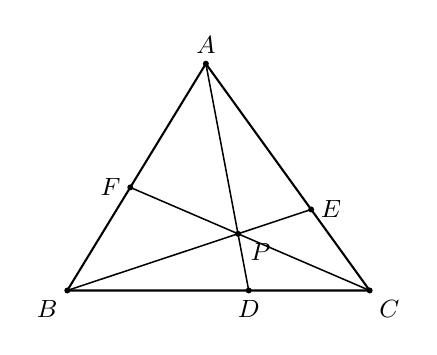
\begin{tikzpicture}[scale=0.80, line cap=round, line join=round, every node/.style={font=\small}]
    \coordinate (A) at (0,3.6);
    \coordinate (B) at (-2.2,0);
    \coordinate (C) at (2.6,0);
    \coordinate (D) at ({17/25},0);
    \coordinate (E) at ({117/70},{9/7});
    \coordinate (F) at ({-6/5},{18/11});
    \coordinate (P) at (0.51,0.9);
    \draw[line width=0.75pt] (A)--(B)--(C)--cycle;
    \draw[line width=0.55pt] (A)--(D) (B)--(E) (C)--(F);
    \foreach \X in {A,B,C,D,E,F,P} {\fill (\X) circle (1.35pt);}
    \node[above] at (A) {$A$};
    \node[below left] at (B) {$B$};
    \node[below right] at (C) {$C$};
    \node[below] at (D) {$D$};
    \node[right] at (E) {$E$};
    \node[left] at (F) {$F$};
    \node[below right,xshift=1pt] at (P) {$P$};
\end{tikzpicture}

    \caption{Three concurrent cevians in $\triangle ABC$.}
\end{figure}

\begin{theorem}[Menelaus' Theorem]
Let $D, E, F$ lie on the lines $BC, CA, AB$, respectively, with none a vertex and no two of $D, E, F$ coinciding. Suppose an odd number of $D, E, F$ lie outside their corresponding closed sides. Then $D, E, F$ are collinear if and only if
\[
 \frac{BD}{DC}\frac{CE}{EA}\frac{AF}{FB}=1,
\]
where the numerator and denominator are ordinary (unsigned) lengths. In a collinear configuration with no vertex intersections, the number of exterior points is necessarily odd.
\end{theorem}

\begin{theorem}[Trigonometric Ceva]
For interior cevians $AD, BE, CF$ of $\triangle ABC$,
\[
 \frac{\sin\angle BAD}{\sin\angle DAC}
 \frac{\sin\angle CBE}{\sin\angle EBA}
 \frac{\sin\angle ACF}{\sin\angle FCB}=1
\]
if and only if $AD, BE, CF$ are concurrent.
\end{theorem}

\begin{definition}[Pedal and Orthic Triangles]
Let $P$ be a point in the plane of a nondegenerate triangle $ABC$. The feet of the perpendiculars from $P$ to the lines $BC$, $CA$, and $AB$ form the pedal triangle of $P$ when they are distinct and noncollinear. The pedal triangle of the orthocenter $H$ of an acute triangle is called its orthic triangle.
\end{definition}

\begin{definition}[Barycentric Coordinates]
For a nondegenerate triangle with position vectors $\mathbf{a}, \mathbf{b}, \mathbf{c}$, a point $P$ has barycentric coordinates $(\alpha:\beta:\gamma)$ when
\[
 \mathbf{p}=\frac{\alpha\mathbf{a}+\beta\mathbf{b}+\gamma\mathbf{c}}{\alpha+\beta+\gamma},
 \qquad \alpha+\beta+\gamma\ne0.
\]
The coordinates are homogeneous: multiplying all three by a common nonzero scalar does not change the point.
\end{definition}


\begin{definition}[Classical Triangle Centers]
The \emph{circumcenter} $O$ is the intersection of the perpendicular bisectors; the \emph{incenter} $I$ is the intersection of the internal angle bisectors; the \emph{centroid} $G$ is the intersection of the medians; and the \emph{orthocenter} $H$ is the intersection of the altitudes. The circumcenter and orthocenter need not lie inside the triangle.
\end{definition}

\begin{definition}[Trilinear Coordinates]
For a reference triangle $ABC$ with side lengths $a=BC$, $b=CA$, $c=AB$, the trilinear coordinates $(x:y:z)$ represent a point by its signed distances to the sidelines $BC$, $CA$, $AB$, up to common nonzero scale. The corresponding barycentric coordinates are
\[
 (ax:by:cz).
\]
In particular, the incenter has trilinears $(1:1:1)$ and barycentrics $(a:b:c)$.
\end{definition}

\begin{theorem}[Centroid Ratio]
The three medians of a triangle meet at $G$. If $D$ is the midpoint of $BC$, then $AG:GD=2:1$. With position vectors $\mathbf{a}, \mathbf{b}, \mathbf{c}$ for the vertices,
\[
 \mathbf{g}=\frac{\mathbf{a}+\mathbf{b}+\mathbf{c}}{3}.
\]
\end{theorem}

\begin{theorem}[Euler Line]
For a triangle with circumcenter $O$, centroid $G$, and orthocenter $H$,
\[
 \overrightarrow{OH}=3\overrightarrow{OG}.
\]
Consequently, unless the three points coincide, they are collinear and $OG:GH=1:2$.
\end{theorem}

\begin{theorem}[Orthocenter Reflection Lemma]
Let $H$ be the orthocenter of $\triangle ABC$. The reflection of $H$ across each sideline lies on the circumcircle of $\triangle ABC$. The reflection of $H$ across the midpoint of any side also lies on that circumcircle.
\end{theorem}

\begin{theorem}[Nine-Point Circle]
The midpoints of the sides, the feet of the altitudes, and the midpoints of the segments joining the orthocenter to the vertices lie on one circle. Its center is the midpoint of $OH$, and its radius is $R/2$.
\end{theorem}

\begin{formula}[Euler's Incenter--Circumcenter Formula]
If $O, I$ are the circumcenter and incenter of a triangle, then
\[
 OI^2=R(R-2r).
\]
In particular, $R\ge2r$, with equality exactly for an equilateral triangle.
\end{formula}

\begin{definition}[Excenters and Excircles]
The three external angle bisectors, together with the appropriate internal bisector, determine the excenters $I_a, I_b, I_c$. The $A$-excircle has radius $r_a$ and is tangent to $BC$ and the extensions of $AB, AC$.
\end{definition}

\begin{formula}[Exradii and Contact Lengths]
For the exradii $r_a, r_b, r_c$ of $\triangle ABC$,
\[
 \Delta=r_a(s-a)=r_b(s-b)=r_c(s-c).
\]
If the incircle touches $BC, CA, AB$ at $D, E, F$, respectively, then
\[
 BD=BF=s-b, \quad CD=CE=s-c, \quad AE=AF=s-a.
\]
\end{formula}

\begin{definition}[Isogonal Lines and Isogonal Conjugates]
Two lines through $A$ are \emph{isogonal} in $\angle BAC$ if they are reflections of each other in its angle bisector. Two points $P, Q$ not on the sidelines of $\triangle ABC$ are \emph{isogonal conjugates} when $AP, AQ$ are isogonal at $A$, and likewise at $B$ and $C$.
\end{definition}

\begin{definition}[Isotomic Conjugates]
Two cevians from a vertex are isotomic if their intersections with the opposite sideline are reflections of each other about the midpoint of that side. The cevians isotomic to the three cevians through a point $P$ are concurrent at its isotomic conjugate, when defined. In barycentric coordinates relative to $ABC$,
\[
 (x:y:z)\longmapsto\left(\frac1x:\frac1y:\frac1z\right),
\]
for $xyz\ne0$. The isogonal conjugation is similarly
\[
 (x:y:z)\longmapsto\left(\frac{a^2}x:\frac{b^2}y:\frac{c^2}z\right).
\]
\end{definition}

\begin{theorem}[Symmedian Lemma]
Let $K\in BC$ and suppose $AK$ is the isogonal of the median from $A$. Then
\[
 \frac{BK}{KC}=\frac{AB^2}{AC^2}.
\]
The three symmedians are concurrent at the symmedian point (Lemoine point).
\end{theorem}

\begin{proposition}[Barycentric Coordinates of Triangle Centers]
Relative to $\triangle ABC$, the centroid and incenter have barycentric coordinates
\[
 G=(1:1:1), \qquad I=(a:b:c),
\]
where $a=BC$, $b=CA$, $c=AB$. The symmedian point has coordinates $(a^2:b^2:c^2)$.
\end{proposition}

\begin{theorem}[Gergonne and Nagel Points]
The cevians from the vertices to the points of tangency of the incircle with the opposite sides are concurrent at the \emph{Gergonne point}. The cevians to the points of tangency of the corresponding excircles with the opposite sides are concurrent at the \emph{Nagel point}.
\end{theorem}

\begin{theorem}[Feuerbach's Theorem]
The nine-point circle of a non-equilateral triangle is internally tangent to its incircle and externally tangent to each of its three excircles. For an equilateral triangle, the nine-point circle and incircle coincide.
\end{theorem}

\begin{theorem}[Fermat--Torricelli Point]
If all angles of $\triangle ABC$ are less than $120^\circ$, there is a unique point $P$ minimizing $PA+PB+PC$, characterized by
\[
 \angle APB=\angle BPC=\angle CPA=120^\circ.
\]
If one angle is at least $120^\circ$, its vertex minimizes that sum.
\end{theorem}

\begin{formula}[Half-Angle Relations in a Triangle]
For $s=(a+b+c)/2$ and inradius $r$,
\[
 \tan\frac A2=\frac{r}{s-a}, \qquad
 \sin\frac A2=\sqrt{\frac{(s-b)(s-c)}{bc}},
\]
with cyclic analogues. Moreover,
\[
 r=4R\sin\frac A2\sin\frac B2\sin\frac C2.
\]
\end{formula}

\begin{theorem}[Morley's Trisector Theorem]
The three points obtained by intersecting pairs of adjacent internal angle trisectors of any nondegenerate triangle form an equilateral triangle.
\end{theorem}

\begin{theorem}[Napoleon's Theorem]
Construct equilateral triangles externally on the three sides of an arbitrary triangle. Their centers are the vertices of an equilateral triangle. The corresponding statement also holds when all three equilateral triangles are constructed internally.
\end{theorem}

\begin{theorem}[Van Aubel's Theorem]
If squares are constructed externally on the sides of a quadrilateral, the segments joining centers of squares on opposite sides have equal lengths and are perpendicular.
\end{theorem}

\begin{theorem}[Directed-Angle Criterion for Concyclicity]
Let $A, B, C$ be noncollinear points, and let $D$ be distinct from them. The four points are concyclic if and only if
\[
 \angle(\overleftrightarrow{AB}, \overleftrightarrow{AC})\equiv\angle(\overleftrightarrow{DB}, \overleftrightarrow{DC})\pmod\pi,
\]
where the directed angles use the lines determined by the indicated pairs of points.
\end{theorem}

\begin{theorem}[Inscribed Angle and Tangent--Chord Theorems]
An inscribed angle subtending an arc has half the measure of the corresponding central angle. The angle between a tangent to a circle at $A$ and a chord $AB$ equals the inscribed angle subtending chord $AB$, with directed angles interpreted modulo $\pi$.
\end{theorem}

\begin{theorem}[Cyclic Quadrilateral Criterion]
A convex quadrilateral $ABCD$ is cyclic if and only if
\[
 \angle ABC+\angle ADC=180^\circ.
\]
Equivalently, its opposite angles are supplementary. With directed angles, cyclicity may be characterized without assuming convexity.
\end{theorem}

\begin{formula}[Equation of a Circle and Radical Axis]
In Cartesian coordinates a circle with center $(a,b)$ and radius $r>0$ has equation
\[
 (x-a)^2+(y-b)^2=r^2.
\]
For two circles written in the form
\[
 x^2+y^2+D_ix+E_iy+F_i=0\quad(i=1,2),
\]
their radical axis, when the centers differ, is the line
\[
 (D_1-D_2)x+(E_1-E_2)y+F_1-F_2=0.
\]
This is the locus of points having equal power with respect to the two circles.
\end{formula}

\begin{theorem}[Power of a Point]
For a circle $\omega$ with center $O$ and radius $R$, define
\[
 \PointPower_{\omega}(P)=PO^2-R^2.
\]
If a line through $P$ intersects the circle at $A, B$, let $t_A, t_B$ be the signed coordinates of $A, B$ along that line, measured from $P$ in a common orientation. Then
\[
 t_At_B=\PointPower_{\omega}(P).
\]
In particular, for external secants, the ordinary positive lengths satisfy $PA\cdot PB=PC\cdot PD$. For a tangent $PT$,
\[
 PT^2=\PointPower_{\omega}(P).
\]
\end{theorem}

\begin{theorem}[Radical Axis and Radical Center]
For two distinct nonconcentric circles $\omega_1, \omega_2$, the locus of points satisfying
\[
 \PointPower_{\omega_1}(P)=\PointPower_{\omega_2}(P)
\]
is a line perpendicular to their line of centers, called the \emph{radical axis}. For three circles whose centers are not collinear, the pairwise radical axes are concurrent at their \emph{radical center}.
\end{theorem}

\begin{definition}[Coaxal Circles]
A family of circles is coaxal if every pair of distinct nonconcentric members has the same radical axis. A circle with equation
\[
 x^2+y^2+D x+E y+F=0
\]
belongs to the coaxal family determined by two distinct circles $S_1=0$ and $S_2=0$ precisely when its equation can be written as $S_1+t(S_2-S_1)=0$ for a real parameter $t$, whenever the resulting real locus is a nondegenerate circle. Any three circles in a coaxal family have a common radical axis.
\end{definition}


\begin{figure}[htbp]
    \centering
    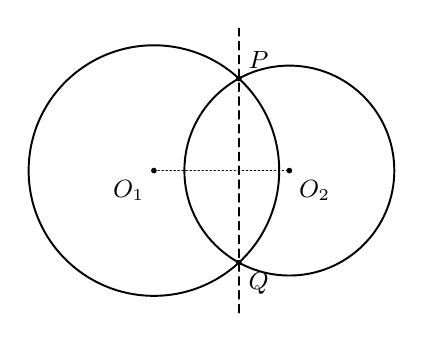
\begin{tikzpicture}[scale=0.86, line cap=round, line join=round, every node/.style={font=\small}]
    \coordinate (O1) at (-1,0);
    \coordinate (O2) at (1,0);
    \coordinate (P) at ({51/200},{sqrt(1.847475)});
    \coordinate (Q) at ({51/200},{-sqrt(1.847475)});
    \draw[line width=0.70pt] (O1) circle (1.85);
    \draw[line width=0.70pt] (O2) circle (1.55);
    \draw[densely dashed,line width=0.5pt] ({51/200},-2.1)--({51/200},2.1);
    \draw[densely dotted,line width=0.45pt] (O1)--(O2);
    \foreach \X in {O1,O2,P,Q} {\fill (\X) circle (1.2pt);}
    \node[below left] at (O1) {$O_1$};
    \node[below right] at (O2) {$O_2$};
    \node[above right] at (P) {$P$};
    \node[below right] at (Q) {$Q$};
\end{tikzpicture}

    \caption{The radical axis of two intersecting circles is their common chord line.}
\end{figure}

\begin{theorem}[Ptolemy's Theorem and Inequality]
For a convex cyclic quadrilateral $ABCD$,
\[
 AC\cdot BD=AB\cdot CD+BC\cdot DA.
\]
For any four points in the Euclidean plane, the corresponding inequality
\[
 AC\cdot BD\le AB\cdot CD+BC\cdot DA
\]
holds. For four distinct vertices in convex order, equality characterizes cyclicity.
\end{theorem}

\begin{formula}[Brahmagupta's Formula]
For a convex cyclic quadrilateral with side lengths $a, b, c, d$ and semiperimeter $s=(a+b+c+d)/2$, its area $K$ satisfies
\[
 K=\sqrt{(s-a)(s-b)(s-c)(s-d)}.
\]
\end{formula}

\begin{theorem}[Pitot's Theorem]
If a convex quadrilateral $ABCD$ has an incircle tangent to all four sides, then
\[
 AB+CD=BC+DA.
\]
This equality alone does not characterize tangential quadrilaterals without additional hypotheses.
\end{theorem}

\begin{theorem}[Varignon's Theorem]
The midpoints of the sides of any quadrilateral form a parallelogram. Its area is half the area of the original quadrilateral when the original quadrilateral is simple.
\end{theorem}

\begin{theorem}[Simson Line]
A point $P$ lies on the circumcircle of a triangle $ABC$ if and only if its perpendicular projections onto the three side lines $AB, BC, CA$ are collinear, provided the triangle is nondegenerate. Their common line is called the \emph{Simson line} of $P$.
\end{theorem}

\begin{theorem}[Reim's Theorem]
Let two circles meet at distinct points $P, Q$. Suppose a line through $P$ meets the circles again at $A, B$, and a line through $Q$ meets them again at $C, D$, with $A, C$ on the first circle and $B, D$ on the second. Then $AC\parallel BD$.
\end{theorem}

\begin{theorem}[Miquel's Theorem]
Let $D\in BC$, $E\in CA$, and $F\in AB$ be points distinct from the vertices of $\triangle ABC$. The three circumcircles of $AEF$, $BFD$, and $CDE$ pass through a common point (their \emph{Miquel point}), apart from possible pairwise shared vertices.
\end{theorem}

\begin{definition}[Direct Similarity and Spiral Similarity]
An orientation-preserving similarity of the complex plane has the form
\[
 z\longmapsto az+b, \qquad a\in\C\setminus\{0\}, \ b\in\C.
\]
If $a\ne1$, it has a unique fixed point $z_0=b/(1-a)$ and is a rotation followed by a homothety centered at $z_0$. If $a=1$, it is a translation. The former case is commonly called a \emph{spiral similarity}.
\end{definition}

\begin{definition}[Homothety]
For a point $O$ and a real scalar $k\ne0$, the homothety with center $O$ and ratio $k$ maps a point $X$ to $X'$ satisfying
\[
 \overrightarrow{OX'}=k\overrightarrow{OX}.
\]
It multiplies all distances by $|k|$ and areas by $k^2$.
\end{definition}

\begin{definition}[Inversion in a Circle]
Fix a circle with center $O$ and radius $r>0$. Inversion sends $P\ne O$ to $P'$ on the ray $OP$ with $OP\cdot OP'=r^2$; it is an involution. A line through $O$ maps to itself (with $O$ omitted), and a line not through $O$ maps to a circle through $O$ (with $O$ omitted). A circle through $O$ maps to a line not through $O$; a circle not through $O$ maps to another circle not through $O$.
\end{definition}

\begin{proposition}[Inversion Distance Identity]
Under inversion with center $O$ and radius $r$, for $P, Q\ne O$ with images $P', Q'$,
\[
 P'Q'=\frac{r^2}{OP\cdot OQ}\, PQ.
\]
Inversion preserves the magnitude of angles between intersecting smooth curves, but reverses their orientation.
\end{proposition}

\begin{theorem}[Butterfly Theorem]
Let $M$ be the midpoint of a chord $PQ$ of a circle. Let chords $AB$ and $CD$ pass through $M$, with $A, C$ on one side of $PQ$ and $B, D$ on the other. If $AD$ and $BC$ meet the line $PQ$ at $X$ and $Y$, respectively, then $M$ is the midpoint of $XY$.
\end{theorem}

\begin{proposition}[Circles Orthogonal to an Inversion Circle]
A circle $\omega$ not passing through the center $O$ of an inversion circle is invariant as a set under that inversion if and only if it is orthogonal to the inversion circle, meaning that their tangent lines at either intersection point are perpendicular.
\end{proposition}

\begin{definition}[Projective Plane and Homogeneous Coordinates]
The real projective plane $\mathbb{RP}^2$ consists of one-dimensional linear subspaces of $\R^3$. A point is represented by nonzero homogeneous coordinates $[x:y:z]$, with nonzero scalar multiples identified. The affine plane embeds by $(x,y)\mapsto[x:y:1]$, while $z=0$ is the line at infinity. Two distinct projective lines meet at a unique projective point.
\end{definition}
\begin{proposition}[Projective Collinearity Criterion]
Three points $[x_i:y_i:z_i]\in\mathbb{RP}^2$, $i=1,2,3$, are collinear if and only if
\[
 \det\begin{pmatrix}
 x_1&y_1&z_1\\ x_2&y_2&z_2\\ x_3&y_3&z_3
 \end{pmatrix}=0.
\]
A projective line has an equation $ax+by+cz=0$ for some nonzero $(a,b,c)$, determined up to a nonzero scalar.
\end{proposition}

\begin{definition}[Cross Ratio]
For four distinct collinear points $A, B, C, D$ on a projective line, their cross ratio in an affine coordinate $t$ is
\[
 (A, B;C, D)=\frac{(t_C-t_A)(t_D-t_B)}{(t_C-t_B)(t_D-t_A)},
\]
with the usual limiting interpretation when one point is at infinity. Projective transformations preserve the cross ratio.
\end{definition}

\begin{definition}[Harmonic Range and Harmonic Division]
Four distinct points $A,B,C,D$ on a projective line form a harmonic range if their cross ratio satisfies
\[
 (A,B;C,D)=-1.
\]
Equivalently, $C,D$ are harmonic conjugates with respect to $A,B$.
\end{definition}

\begin{definition}[Complete Quadrangle and Complete Quadrilateral]
A complete quadrangle consists of four points with no three collinear and the six joining lines. Its three diagonal points are intersections of pairs of opposite sides. Dually, a complete quadrilateral consists of four lines with no three concurrent, their six intersections, and the three lines joining opposite intersections.
\end{definition}

\begin{theorem}[Harmonic Property of a Complete Quadrangle]
For four points $A,B,C,D$ in general position, let $X=AB\cap CD$, $Y=AC\cap BD$, and $Z=AD\cap BC$ in the projective plane. The line $YZ$ meets $AB$ at $T$. Then the four collinear points $(A,B;X,T)$ form a harmonic range:
\[
 (A,B;X,T)=-1.
\]
\end{theorem}

\begin{theorem}[Desargues' Theorem]
In the real projective plane, if two triangles have corresponding vertices joined by three concurrent lines, then the intersections of corresponding sides are collinear. Conversely, if the three side intersections are collinear, then the lines joining corresponding vertices are concurrent in the projective plane.
\end{theorem}

\begin{theorem}[Pappus' Theorem]
Let $A, B, C$ lie on one line and $A', B', C'$ on another, with all pairwise intersections below defined. Then the three points
\[
 AB'\cap A'B, \quad AC'\cap A'C, \quad BC'\cap B'C
\]
are collinear in the real projective plane.
\end{theorem}

\begin{definition}[Conic in the Projective Plane]
A nondegenerate projective conic is the zero set of a homogeneous quadratic form in $[x:y:z]\in\mathbb{RP}^2$ whose associated symmetric $3\times3$ matrix is nonsingular. In affine coordinates, ellipses, parabolas, and hyperbolas are the standard nonsingular real conics.
\end{definition}

\begin{definition}[Pole and Polar with Respect to a Conic]
Let a nondegenerate conic in the real projective plane have homogeneous equation $\mathbf{x}^{\mathrm{T}}\mathbf{Q}\mathbf{x}=0$, where $\mathbf{Q}$ is an invertible symmetric $3\times3$ matrix. The polar of a point $[\mathbf{p}]$ is the line
\[
 \mathbf{p}^{\mathrm{T}}\mathbf{Q}\mathbf{x}=0.
\]
Every projective line has a unique pole. For a point $P$ on the conic, its polar is its tangent. Polarity satisfies La Hire's reciprocity: $P$ lies on the polar of $Q$ if and only if $Q$ lies on the polar of $P$.
\end{definition}

\begin{theorem}[La Hire's Theorem]
For a nondegenerate projective conic, the pole of the line through two distinct points $P,Q$ is the intersection of the polars of $P,Q$, provided those polars are distinct. Dually, the polar of the intersection of two distinct lines is the line through their poles.
\end{theorem}

\begin{theorem}[Pascal's Theorem]
For six distinct points $A, B, C, D, E, F$ on a nondegenerate conic, the three intersections of opposite sides
\[
 AB\cap DE, \qquad BC\cap EF, \qquad CD\cap FA
\]
are collinear in the projective plane, allowing points at infinity for parallel sides.
\end{theorem}

\begin{theorem}[Brianchon's Theorem]
For a nondegenerate conic, let $A_1A_2A_3A_4A_5A_6$ be a hexagon whose six sides are tangent to the conic, with consecutive sides meeting at the named vertices. The three principal diagonals
\[
 A_1A_4,\qquad A_2A_5,\qquad A_3A_6
\]
are concurrent in the projective plane.
\end{theorem}


\begin{formula}[Coordinate and Shoelace Area Formulas]
For $A=(x_1, y_1)$, $B=(x_2, y_2)$, $C=(x_3, y_3)$,
\[
 [ABC]=\frac12\left|\det\begin{pmatrix}
 x_2-x_1&y_2-y_1\\ x_3-x_1&y_3-y_1
 \end{pmatrix}\right|.
\]
For a simple polygon with cyclically ordered vertices $(x_i, y_i)$, $1\le i\le n$,
\[
 \operatorname{Area}=\frac12\left|\sum_{i=1}^n(x_iy_{i+1}-x_{i+1}y_i)\right|,
 \quad (x_{n+1}, y_{n+1})=(x_1, y_1).
\]
\end{formula}

\begin{definition}[Eccentricity and Focus--Directrix Property]
A conic with focus $F$, directrix line $\ell$, and eccentricity $e>0$ is the locus of points $P$ satisfying
\[
 PF=e\,d(P,\ell).
\]
For $0<e<1$ it is an ellipse, for $e=1$ a parabola, and for $e>1$ a hyperbola, in the nondegenerate cases. The circle is the special case of an ellipse with equal semiaxes and eccentricity $0$.
\end{definition}

\begin{formula}[Standard Equations of Conic Sections]
For $a>b>0$ and $c^2=a^2-b^2$, an ellipse centered at the origin with major axis on the $x$-axis is
\[
 \frac{x^2}{a^2}+\frac{y^2}{b^2}=1,\qquad
 F_\pm=(\pm c,0),\qquad e=\frac ca.
\]
For $a,b>0$ and $c^2=a^2+b^2$, the corresponding hyperbola is
\[
 \frac{x^2}{a^2}-\frac{y^2}{b^2}=1,\qquad
 F_\pm=(\pm c,0),\qquad e=\frac ca,
\]
with asymptotes $y=\pm(b/a)x$. A parabola with vertex at the origin, focus $(p,0)$, and directrix $x=-p$, where $p\ne0$, is $y^2=4px$.
\end{formula}

\begin{formula}[Tangents to Standard Conics]
For a point $(x_0,y_0)$ on the indicated conic, its tangent line is
\[
 \frac{xx_0}{a^2}+\frac{yy_0}{b^2}=1
 \quad\text{for }\frac{x^2}{a^2}+\frac{y^2}{b^2}=1,
\]
\[
 \frac{xx_0}{a^2}-\frac{yy_0}{b^2}=1
 \quad\text{for }\frac{x^2}{a^2}-\frac{y^2}{b^2}=1,
\]
\[
 yy_0=2p(x+x_0)
 \quad\text{for }y^2=4px\ (p\ne0).
\]
The tangent at $(x_0,y_0)$ to $x^2+y^2=r^2$ is $xx_0+yy_0=r^2$.
\end{formula}


\begin{formula}[Complex Coordinates on the Unit Circle]
For distinct points $a, b, c, d\in\C$ with $|a|=|b|=|c|=|d|=1$,
\[
 \frac{a-b}{c-d}=\frac{ab}{cd}\,
 \overline{\left(\frac{a-b}{c-d}\right)}.
\]
If $a, b, c, d$ are four distinct points on the unit circle, then their complex cross ratio
\[
 \frac{(a-c)(b-d)}{(a-d)(b-c)}
\]
is real.
\end{formula}

\begin{theorem}[Pick's Theorem]
For a simple lattice polygon in $\R^2$, with $I$ lattice points in its interior and $B$ lattice points on its boundary,
\[
 \operatorname{Area}=I+\frac B2-1.
\]
\end{theorem}

\begin{theorem}[Helly's Theorem in the Plane]
Let $\mathcal{F}$ be a finite family of convex subsets of $\R^2$ with at least three members. If every three members have a common point, then all members have a common point.
\end{theorem}

\begin{theorem}[Carath\'eodory's Theorem in the Plane]
If $x$ belongs to the convex hull of a set $S\subseteq\R^2$, then $x$ is a convex combination of at most three points of $S$.
\end{theorem}

\begin{theorem}[Isoperimetric Inequality in the Plane]
Let a simple closed rectifiable curve in the plane have length $L$ and enclose area $A$. Then
\[
 L^2\ge4\pi A,
\]
with equality if and only if the curve is a circle.
\end{theorem}

\begin{definition}[Lines and Planes in Three Dimensions]
Let $\mathbf{p},\mathbf{v},\mathbf{n}\in\R^3$, with $\mathbf{v}\ne\mathbf0$ and $\mathbf{n}\ne\mathbf0$. The line through $\mathbf{p}$ with direction $\mathbf{v}$ is
\[
 \mathbf{x}=\mathbf{p}+t\mathbf{v}\quad(t\in\R),
\]
while the plane through $\mathbf{p}$ with normal $\mathbf{n}$ is
\[
 \mathbf{n}\cdot(\mathbf{x}-\mathbf{p})=0.
\]
Two planes are perpendicular if their normal vectors are perpendicular; they are parallel if their normal vectors are proportional.
\end{definition}
\begin{formula}[Distances and Angles in Space]
Let $\Pi$ be the plane $ax+by+cz+d=0$, with $(a,b,c)\ne(0,0,0)$. For $P=(x_0,y_0,z_0)$,
\[
 \dist(P,\Pi)=\frac{|ax_0+by_0+cz_0+d|}{\sqrt{a^2+b^2+c^2}}.
\] For nonzero direction vectors $\mathbf{u},\mathbf{v}$, the smaller angle $\theta\in[0,\pi/2]$ between their unoriented lines satisfies
\[
 \cos\theta=\frac{|\mathbf{u}\cdot\mathbf{v}|}{\|\mathbf{u}\|\|\mathbf{v}\|}.
\]
The distance from $\mathbf{p}$ to the line $\mathbf{a}+t\mathbf{v}$ is $\|(\mathbf{p}-\mathbf{a})\times\mathbf{v}\|/\|\mathbf{v}\|$.
\end{formula}
\begin{formula}[Vector Products and Tetrahedron Volume]
For $\mathbf{u},\mathbf{v},\mathbf{w}\in\R^3$, the area of the parallelogram spanned by $\mathbf{u},\mathbf{v}$ is $\|\mathbf{u}\times\mathbf{v}\|$, and the volume of the corresponding parallelepiped is
\[
 |\mathbf{u}\cdot(\mathbf{v}\times\mathbf{w})|.
\]
For tetrahedron $ABCD$ with position vectors $\mathbf{a},\mathbf{b},\mathbf{c},\mathbf{d}$, its volume is
\[
 \frac16\left|\det\begin{pmatrix}
 b_1-a_1&c_1-a_1&d_1-a_1\\
 b_2-a_2&c_2-a_2&d_2-a_2\\
 b_3-a_3&c_3-a_3&d_3-a_3
 \end{pmatrix}\right|.
\]
\end{formula}

\begin{formula}[Basic Solid Geometry]
A right circular cylinder of radius $r$ and height $h$ has volume $\pi r^2h$; a right circular cone has volume $\pi r^2h/3$; and a ball of radius $r$ has volume $4\pi r^3/3$ and boundary area $4\pi r^2$.
\end{formula}

\begin{theorem}[Euler's Polyhedron Formula]
For a convex polyhedron with $V$ vertices, $E$ edges, and $F$ faces,
\[
 V-E+F=2.
\]
The same identity holds for a connected planar graph in a plane embedding when the unbounded face is included.
\end{theorem}

\begin{theorem}[Cavalieri's Principle]
Two measurable plane regions having equal cross-sectional lengths at almost every level in a fixed direction have equal area, provided their areas are finite. Similarly, solids with equal cross-sectional areas at almost every height have equal volume when the volumes are finite.
\end{theorem}
